% Generated by render.py; edit preamble.tex, citations.json and relations.tikz
\documentclass[border=12pt]{standalone}
\def\pgfsysdriver{pgfsys-dvisvgm.def}
\usepackage[dvisvgm]{xcolor}
\usepackage{xeCJK}
\setCJKmainfont{HaranoAjiGothic-Regular.otf}[BoldFont=HaranoAjiGothic-Bold.otf]
\setCJKsansfont{HaranoAjiGothic-Regular.otf}[BoldFont=HaranoAjiGothic-Bold.otf]
\usepackage{amsmath,amssymb,tikz,lmodern}
\usetikzlibrary{arrows.meta,positioning,calc,fit,backgrounds}
\renewcommand{\familydefault}{\sfdefault}
\definecolor{ink}{HTML}{25322F}
\definecolor{green}{HTML}{246657}
\definecolor{tint}{HTML}{EEF4F0}
\definecolor{soft}{HTML}{C6D2CC}
\definecolor{muted}{HTML}{52615B}
\newif\ifJapanese
\newcommand{\Tx}[2]{\ifJapanese #1\else #2\fi}
\newcommand{\Eff}{\overline{\operatorname{Eff}}}
\newcommand{\heading}[3]{{\color{green}\bfseries #1\quad\Tx{#2}{#3}}\\[5pt]}
% A white rectangle makes the complete citation label clickable, including spaces.
\newcommand{\refurl}[2]{\special{dvisvgm:raw <a xlink:href="#1" target="_blank" rel="noopener noreferrer">}{\setlength{\fboxsep}{0pt}\colorbox{white}{\color{green}\underline{\strut #2}}}\special{dvisvgm:raw </a>}}
\tikzset{
 card/.style={draw=soft,fill=white,rounded corners=2pt,align=left,text=ink,font=\fontsize{10.5}{14}\selectfont,inner xsep=12pt,inner ysep=10pt,text width=14.4cm},
 half/.style={card,text width=6.45cm,minimum height=2.05cm},
 result/.style={card,draw=green,fill=tint,line width=.9pt},
 reason/.style={align=left,text=muted,font=\fontsize{9}{12}\selectfont,inner sep=0pt,text width=12.6cm},
 branchreason/.style={reason,text width=5.95cm},
 edge/.style={-{Stealth[length=2.4mm]},draw=green,line width=1pt},
 wire/.style={draw=green,line width=1pt},
}
% Keep the arrow in a dedicated left gutter; explanations never cover it.
\def\flow#1#2#3;{
 \coordinate (#2-from) at ($(#1.south)+(-6.9,0)$);
 \coordinate (#2-to) at ($(#2.north)+(-6.9,0)$);
 \draw[edge] (#2-from)--(#2-to);
 \node[reason,anchor=west] (#2-reason) at ($(#2-from)!.5!(#2-to)+(.55,0)$) {#3};
}

% Style adapted from the repository's Schnell diagrams; MIT attribution retained.

% Generated from citations.json; do not edit.
\newcommand{\Cite}[1]{\csname cite-#1\endcsname}
\expandafter\def\csname cite-official\endcsname{\shortstack[l]{\refurl{https://github.com/openai/math/blob/1581d4cbdd69a0faf34b2089614fe2a814316a6a/overview.pdf}{OpenAI Research Catalog · 039 · p. 6}}}
\expandafter\def\csname cite-plane\endcsname{\shortstack[l]{\refurl{https://github.com/openai/math/blob/1581d4cbdd69a0faf34b2089614fe2a814316a6a/preprints/Nagatas-Conjecture-for-Plane-Curves-September-23-2026/main.pdf}{[OpenAI26a, Theorem 1.1; Corollary 6.2, pp. 1, 22]}}}
\expandafter\def\csname cite-surface\endcsname{\shortstack[l]{\refurl{https://github.com/openai/math/blob/1581d4cbdd69a0faf34b2089614fe2a814316a6a/preprints/Maximal-Seshadri-Constants-on-Arbitrary-Polarized-Surfaces-September-23-2026/main.pdf}{[OpenAI26b, Theorem 1.1; Corollary 5.5, pp. 2, 18]}}}
\expandafter\def\csname cite-higher\endcsname{\shortstack[l]{\refurl{https://github.com/openai/math/blob/1581d4cbdd69a0faf34b2089614fe2a814316a6a/preprints/Maximal-Multipoint-Seshadri-Constants-in-Higher-Dimensions-October-5-2026/main.pdf}{[OpenAI26c, Theorem 1.1, pp. 1–2]}}}
\expandafter\def\csname cite-positive\endcsname{\shortstack[l]{\refurl{https://github.com/openai/math/blob/1581d4cbdd69a0faf34b2089614fe2a814316a6a/preprints/Maximal-multipoint-Seshadri-constants-in-positive-characteristic-October-5-2026/seshadri-positive-characteristic.pdf}{[OpenAI26d, Theorem 1.1; Remark 6.3, pp. 1–2, 16]}}}
\expandafter\def\csname cite-surface-method\endcsname{\shortstack[l]{\refurl{https://github.com/openai/math/blob/1581d4cbdd69a0faf34b2089614fe2a814316a6a/preprints/Maximal-Seshadri-Constants-on-Arbitrary-Polarized-Surfaces-September-23-2026/main.pdf}{[OpenAI26b, Propositions 3.2, 3.4; Lemma 4.3, pp. 8–10, 14]}}}
\expandafter\def\csname cite-higher-method\endcsname{\shortstack[l]{\refurl{https://github.com/openai/math/blob/1581d4cbdd69a0faf34b2089614fe2a814316a6a/preprints/Maximal-Multipoint-Seshadri-Constants-in-Higher-Dimensions-October-5-2026/main.pdf}{[OpenAI26c, §1.1; Proposition 4.1, pp. 2, 9–14]}}}
\expandafter\def\csname cite-positive-method\endcsname{\shortstack[l]{\refurl{https://github.com/openai/math/blob/1581d4cbdd69a0faf34b2089614fe2a814316a6a/preprints/Maximal-multipoint-Seshadri-constants-in-positive-characteristic-October-5-2026/seshadri-positive-characteristic.pdf}{[OpenAI26d, §1.1; §4; §5, pp. 2, 8–14]}}}

\Japanesefalse
\begin{document}
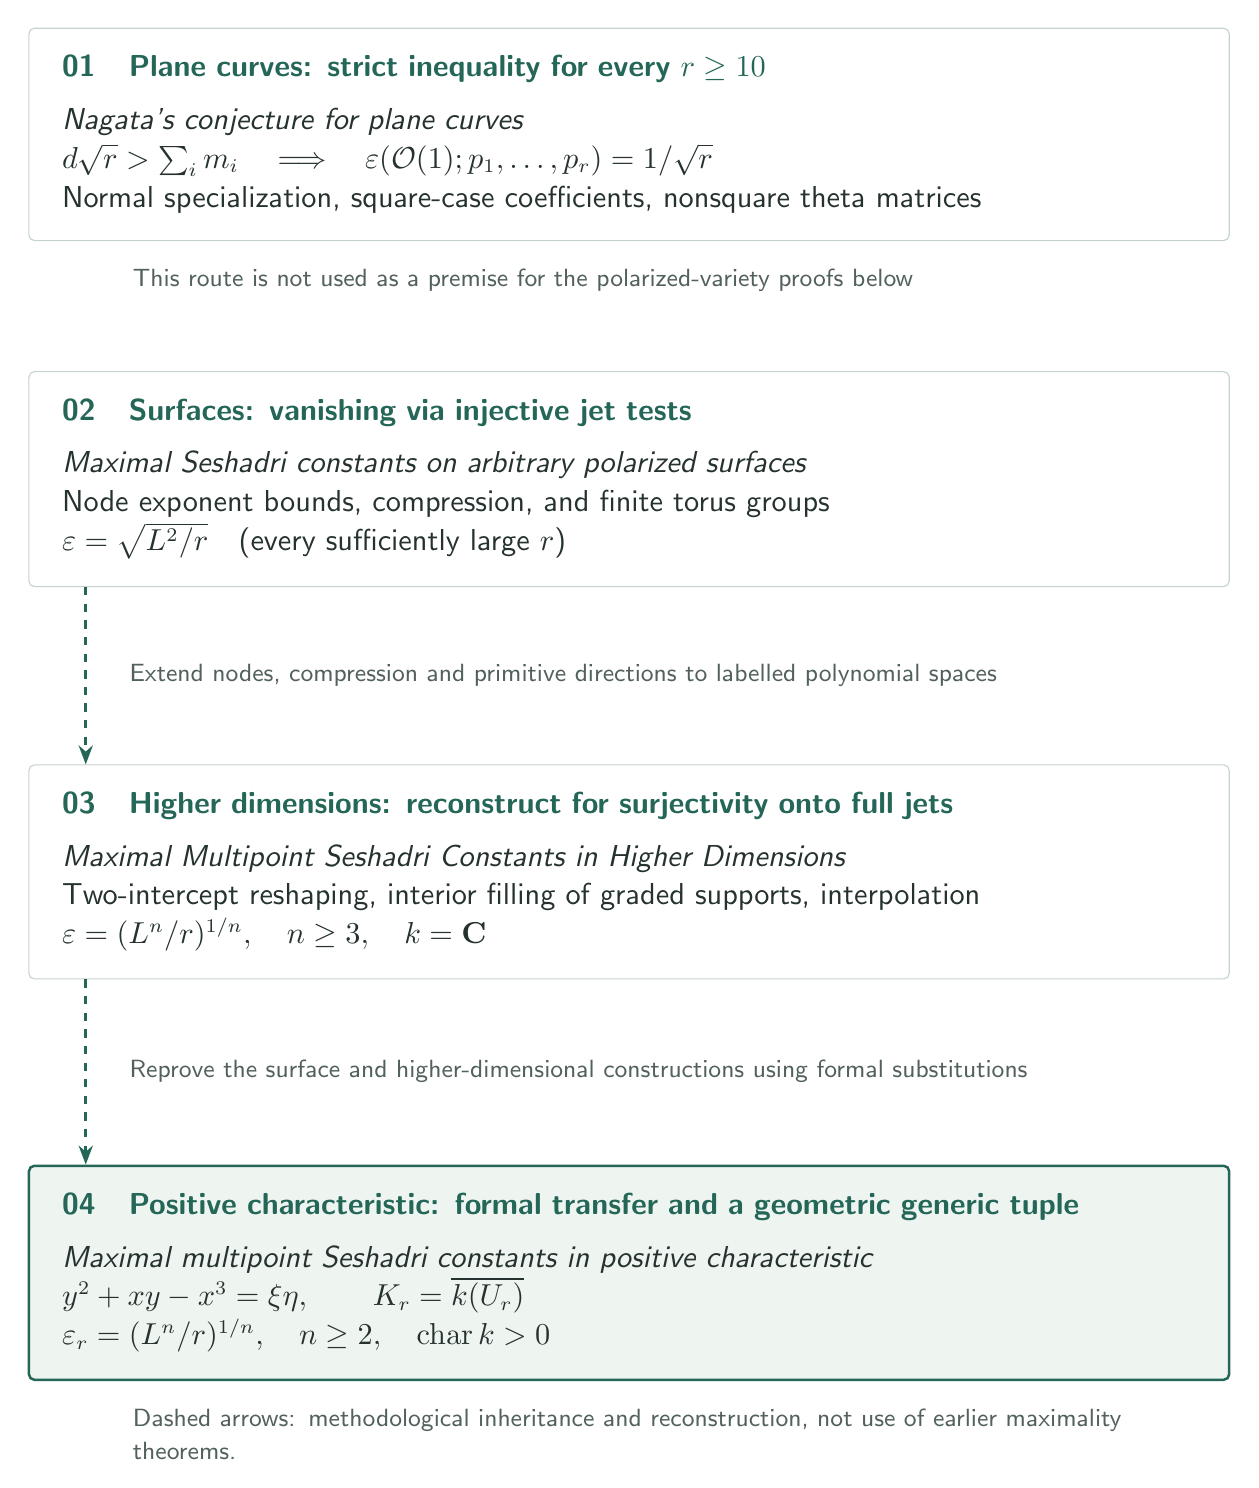
\begin{tikzpicture}
\node[card] (plane) {\heading{01}{平面曲線：全 $r\geq10$ の厳密不等式}{Plane curves: strict inequality for every $r\geq10$}
\textit{Nagata's conjecture for plane curves}\\
$d\sqrt r>\sum_i m_i\quad\Longrightarrow\quad\varepsilon(\mathcal O(1);p_1,\ldots,p_r)=1/\sqrt r$\\
\Tx{法束への特殊化、平方数の係数比較、非平方数のtheta行列}{Normal specialization, square-case coefficients, nonsquare theta matrices}};
\node[reason,below=0.35cm of plane] (note) {\Tx{この経路を、下の一般偏極多様体の証明へ接続しない}{This route is not used as a premise for the polarized-variety proofs below}\\\Cite{plane}};
\node[card,below=1.65cm of plane] (surface) {\heading{02}{曲面：jet単射性による消滅}{Surfaces: vanishing via injective jet tests}
\textit{Maximal Seshadri constants on arbitrary polarized surfaces}\\
\Tx{節点の指数境界・圧縮・有限トーラス群}{Node exponent bounds, compression, and finite torus groups}\\
$\varepsilon=\sqrt{L^2/r}$\quad\Tx{（十分大きい全 $r$）}{(every sufficiently large $r$)}};
\node[card,below=2.25cm of surface] (higher) {\heading{03}{高次元：全jetへの全射性へ作り直す}{Higher dimensions: reconstruct for surjectivity onto full jets}
\textit{Maximal Multipoint Seshadri Constants in Higher Dimensions}\\
\Tx{二切片変形・次数付き支持の内部充填・補間}{Two-intercept reshaping, interior filling of graded supports, interpolation}\\
$\varepsilon=(L^n/r)^{1/n},\quad n\geq3,\quad k=\mathbf C$};
\draw[edge,dashed] ($(surface.south)+(-6.9,0)$)--($(higher.north)+(-6.9,0)$);
\node[reason,anchor=west] at ($(surface.south)+(-6.35,-1.12)$) {\Tx{節点・圧縮・原始格子方向を、ラベル付き多項式空間へ拡張}{Extend nodes, compression and primitive directions to labelled polynomial spaces}\\\Cite{higher-method}};
\node[result,below=2.35cm of higher] (positive) {\heading{04}{正標数：形式的移送と幾何学的一般点}{Positive characteristic: formal transfer and a geometric generic tuple}
\textit{Maximal multipoint Seshadri constants in positive characteristic}\\
$y^2+xy-x^3=\xi\eta,\qquad K_r=\overline{k(U_r)}$\\
$\varepsilon_r=(L^n/r)^{1/n},\quad n\geq2,\quad\operatorname{char}k>0$};
\draw[edge,dashed] ($(higher.south)+(-6.9,0)$)--($(positive.north)+(-6.9,0)$);
\node[reason,anchor=west] at ($(higher.south)+(-6.35,-1.17)$) {\Tx{曲面・高次元の構成を再証明：解析極限を形式代入へ}{Reprove the surface and higher-dimensional constructions using formal substitutions}\\\Cite{positive-method}};
\node[reason,below=0.35cm of positive] {\Tx{破線＝方法の継承・再構成。先行する最大性の主定理の直接入力ではない}{Dashed arrows: methodological inheritance and reconstruction, not use of earlier maximality theorems.}};

\end{tikzpicture}
\end{document}
